\documentclass[xcolor=x11names, svgnames, rgb]{beamer}

\setbeamertemplate{navigation symbols}{}
\setbeamercolor{block title}{bg=blue!40}
\setbeamercolor{block body}{bg=blue!20}

%% Beamer Layout %%%%%%%%%%%%%%%%%%%%%%%%%%%%%%%%%%
\useoutertheme[subsection=false,shadow]{miniframes}
\useinnertheme{default}
\usefonttheme{serif}
\usepackage{palatino}
\setbeamerfont{title like}{shape=\scshape}
\setbeamerfont{frametitle}{shape=\scshape}
\setbeamercolor*{lower separation line head}{bg=DeepSkyBlue4}
\setbeamercolor*{normal text}{fg=black,bg=white}
\setbeamercolor*{alerted text}{fg=red}
\setbeamercolor*{example text}{fg=black}
\setbeamercolor*{structure}{fg=black}
\setbeamercolor*{palette tertiary}{fg=black,bg=black!10}
\setbeamercolor*{palette quaternary}{fg=black,bg=black!10}
%% END Beamer Layout %%%%%%%%%%%%%%%%%%%%%%%%%%%%%%%%%%%%%%%%%%%%
\usepackage{graphicx}
\newcommand{\dom}{\text{AA}}
\newcommand{\het}{\text{Aa}}
\newcommand{\rec}{\text{aa}}
\usepackage{mathtools}



\title{On Equlibria of Allele Frequencies In a Gene Pool - A Simple Simulation }
\author{Alek Westover}
\institute{AP Chemistry}
\date{October 14, 2019}

\begin{document}
 
\frame{\titlepage}

\begin{frame}[t]{The Example of Equilibrium: Allele Frequencies}
	I made a simulation	of how the genotypes of a population will converge over time to an equilibrium (in the simple case that I consider) as a result of selective pressure.\\
	\vspace{0.5cm}
	In my model I consider animals (sheep) that have 2 possible phenotypes (physical characteristics) as determined by 2 alleles (their genotype).\\
	\vspace{0.5cm}
	The phenotype is displayed by the indicator of color, there are black sheep and there are blue sheep.\\

\end{frame}

\begin{frame}[t]{The Genotypes and Corresponding Phenotypes}
	The phenotype is determined by a single gene.\\
	 The organisms gets an allele of the gene from their father and their mother. The black color is dominant. The phenotypes that arise from each genotype are depicted in the following table:
	\begin{center}
	\begin{tabular}{ c | c | c }
	  & A & a \\ 
		\hline
		A & 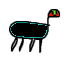
\includegraphics[width=0.15\linewidth]{dogBlack.png} & 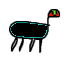
\includegraphics[width=0.15\linewidth]{dogBlack.png} \\  
		\hline
		a & 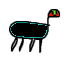
\includegraphics[width=0.15\linewidth]{dogBlack.png} & 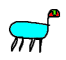
\includegraphics[width=0.15\linewidth]{dogBlue.png} 
	\end{tabular}
	\end{center}
\end{frame}

\begin{frame}[t]{What is the equilibrium that arises?}
	In my first simulation I give each phenotype a certain chance of dying in any given year.	
	For the Black sheep I made this probability 0.2, and for the blue sheep I made this probability 0.1 (Note: this is a very simplistic model). 
	Every year, each sheep that is not dead by the end of the year mates with a random sheep and they produce an offspring. The offspring gets a randomly chosen allele from each of its parents, which determines its phenotype.\\
	After the mating I randomly kill sheep until so that the total sheep
	population is the same as it was the previous year. Note that this should
	essentially preserve the ratios of each genotype as long as the populations
	are big enough. This step is my way of enforcing a carrying capacity in the
	population (without this, sheep are expected to reproduce much more than they
	die off, so my simulation would quickly get really big numbers which would
	make it slow).
\end{frame}

\begin{frame}[t]{Mathematically modelling the Equilibrium}
	Let the total popuation size be $n$. Let $\dom(t), \het(t), \rec(t)$ be the frequencies of the genotypes AA,Aa,aa at year $t$.
	By the end of the year, before the mating, there will be (on average) $0.8 n \dom(t),0.8 n \het(t),0.9 n\rec(t)$ of each genotype of sheep (according to the death probabilities for each phenotype).\\
	Let $f_{AA},f_{Aa},f_{aa}$ be the frequencies of the alleles in the population after the sheep die for the year, before they mate for the year.
\end{frame}

% \begin{frame}[t]{Mating cases}
% Now we must consider all cases of mating.\\

% \begin{itemize}
%   \item When a aa sheep mates, there is a $f_{AA} + 0.5\cdot f_{Aa}$ chance that the offspring is Aa, and a $f_{aa} + 0.5\cdot f_{Aa} $ chance that the offspring is aa (and $0$ chance that the offspring is AA).
%   \item When a Aa sheep mates, there is a $0.5 \cdot (f_{AA}+0.5 \cdot f_{Aa})$ chance that the offspring is an AA, a $0.5 \cdot (f_{aa}+0.5 \cdot f_{Aa})$ chance that the offspring is aa, and a $0.5\cdot (f_{aa} + 0.5\cdot f_{Aa}) + 0.5 \cdot (f_{AA} + 0.5 \cdot f_{Aa})$ chance that the offspring is Aa.
%   \item When a AA sheep mates there is $0$ chance that the offspring is aa, there is $0.5\cdot f_{Aa} + f_{aa}$ chance that the offspring is Aa, and $f_{AA} + 0.5 \cdot f_{Aa}$ chance that the offspring is Aa.
% \end{itemize}
% \end{frame}

% \begin{frame}[t]{Aggregating the Math}
% We then can combine these expressions to determine the expected new makeup of the population.

% \end{frame}

\begin{frame}[t]{Computing the next generation}
	Now we compute the probability of each genotype.
	\begin{itemize}
		\item Probability of aa: $$f_{aa}\cdot f_{aa} + \frac{1}{2}f_{aa}\cdot f_{Aa} + \frac{1}{2}f_{Aa} \cdot f_{aa} + \frac{1}{4} f_{Aa}\cdot f_{Aa}$$
			$$=(f_{aa} + \frac{1}{2}f_{Aa})^2$$
		% \item Probability of Aa: $$\frac{1}{2}f_{Aa}\cdot (f_{aa} + \frac{1}{2} f_{Aa}) + \frac{1}{2}f_{Aa}\cdot (f_{AA} + \frac{1}{2} f_{Aa}) + $$
		\item Probability of AA: $$f_{AA}\cdot f_{AA} + \frac{1}{2}f_{AA}\cdot f_{Aa} + \frac{1}{2}f_{Aa}\cdot f_{AA} + \frac{1}{4}f_{Aa} \cdot f_{Aa}$$
			$$=(f_{AA} + \frac{1}{2}f_{Aa})^2.$$
		\item Probability of Aa: $1-(f_{AA} + \frac{1}{2}f_{Aa})^2 - (f_{aa} + \frac{1}{2}f_{Aa})^2$
	\end{itemize}
\end{frame}

\begin{frame}[t]{Getting Explicit formulas}
	Let $c = 0.8\cdot \dom(t) + 0.8 \het(t) + 0.9 \rec(t)$. Note that $c n$ is the population after the death, and that 
	$$f_{aa} = \frac{0.9 \rec(t)}{c}, f_{Aa} = \frac{0.8 \het(t)}{c}, f_{AA} = \frac{0.8 \dom(t)}{c}.$$
	Let $f_{aa}', f_{AA}', f_{Aa}'$ be the frequencies of the alleles after the death and mating.
	Then
	$$f_{aa}' = \left(\frac{0.9\rec(t) + \frac{1}{2} 0.8 \het(t)}{c}\right)^2$$
	$$f_{AA}' = \left(\frac{0.8\dom(t) + \frac{1}{2} 0.8 \het(t)}{c}\right)^2$$
	$f_{Aa}' = 1 - f_{aa}' - f_{AA}'$
\end{frame}

\begin{frame}[t]{So What?}
	It is not obvious at surface inspection that these formulas imply that an
	equlibrium will ensue. I will create a simulation to get reasonable values
	for these frequencies, and then come back to these equations to see if they
	are stable at the equilibrium point suggested by my simulation.
\end{frame}

\begin{frame}[t]{A Simulation}
	Not surprisingly, aa quickly dominates and the equilibrium is where all sheep are aa. Note that our formula predicts that this is an equilibrium (plug in $\rec(t) = 1, \het(t) = 0, \dom(t) = 0$ and the ratios remain constant)
\begin{center}
	\begin{figure}
		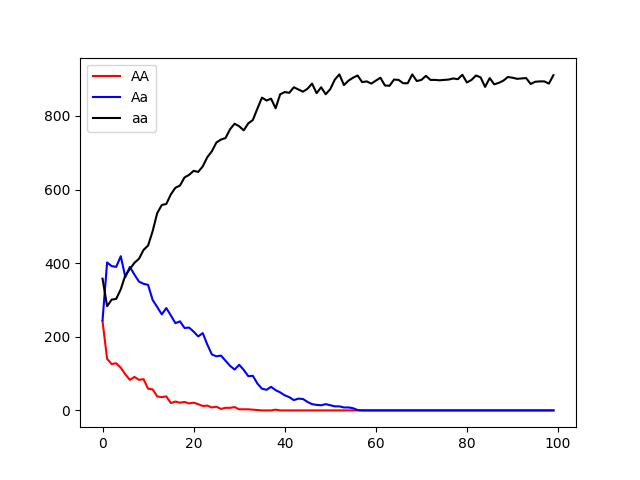
\includegraphics[width=0.7\linewidth]{sim1.png}
\end{figure}	
\end{center}	
\end{frame}

\begin{frame}[t]{Changing the Probabilities}
	If we change the situation so that the black sheep have a 90\% chance of surviving in a year and the blue sheep have a 80\% chance of surviving in the year then the equilibrium becomes all black sheep (specifically AA).

\begin{center}
	\begin{figure}
		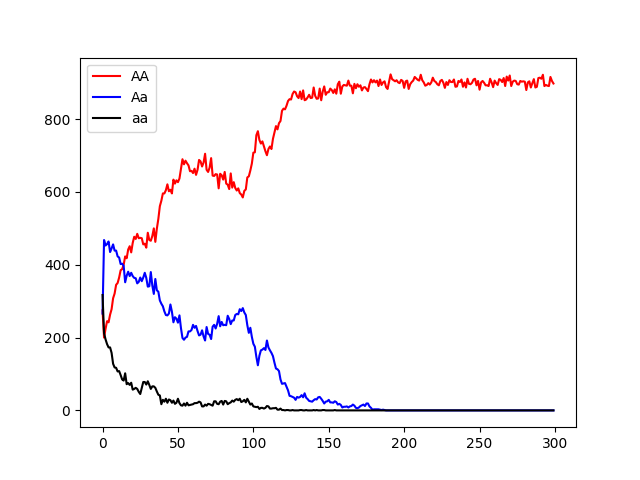
\includegraphics[width=0.7\linewidth]{sim2.png} 
\end{figure}	
\end{center}	
	
\end{frame}

\begin{frame}[t]{A more interesting Equilibrium}
	By making the probability of heterozygotes surviving higher (this could be reasonable because heterozygotes are more flexible) we get the following graph: 

\begin{center}
	\begin{figure}
		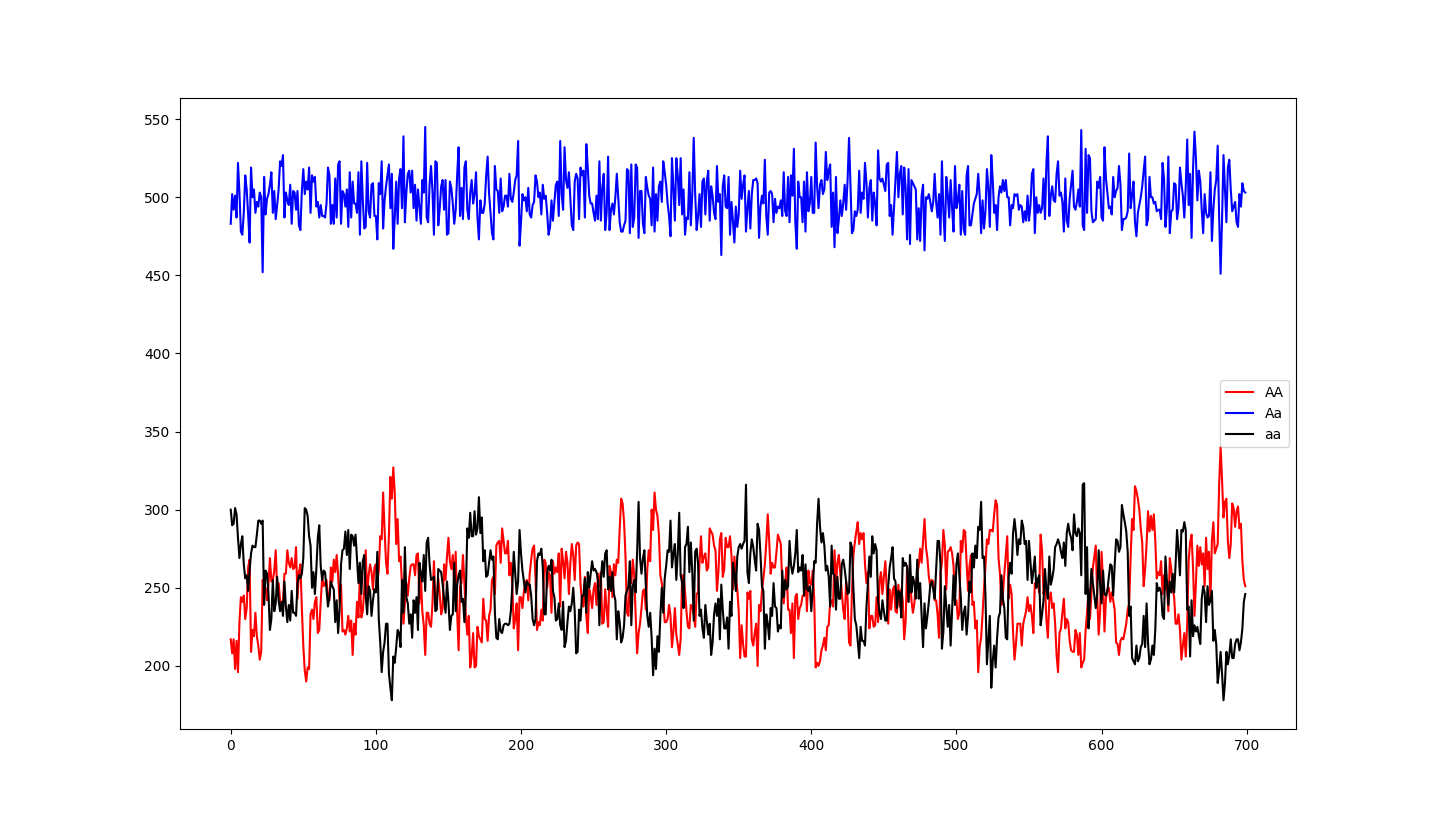
\includegraphics[width=0.6\linewidth]{sim3.png} 
\end{figure}	
\end{center}	
Note that while the populations of AA and aa are in constant flux they stabilize out to being centered around some value, which I call the equilibrium. If the population size were bigger then I imagine that this oscilation would be harder to see.
	
\end{frame}

\begin{frame}[t]{Oscilation at equilibrium is less visible when the population size is larger}
	Here is a graph of what could happen when the probability of AA dying is 30\%, the probability of Aa dying is 10\% and the probabilty of aa dying is 40\% (in a given year):
\begin{center}
	\begin{figure}
		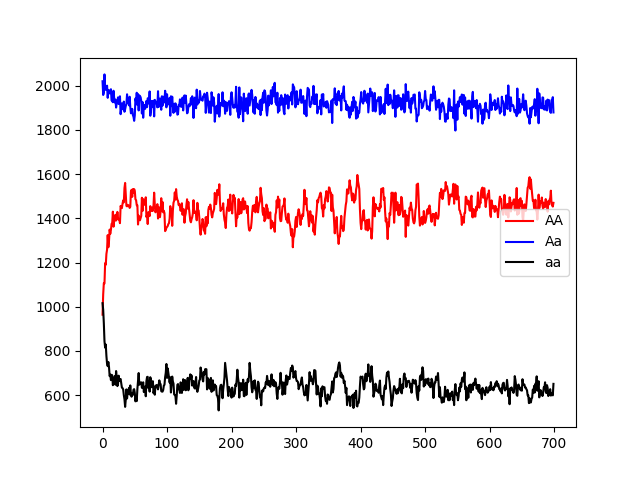
\includegraphics[width=0.6\linewidth]{sim4.png} 
\end{figure}	
\end{center}	
\end{frame}

\begin{frame}[t]{Why does the Equilibrium occur? - Mathematical Answer}
	In the situation described in the previous slide the long run averages of the frequencies of AA, Aa, aa are 0.368836, 0.47636, 0.154804.\\
	Let's plug these into the obvious extension of our formula for $f'_{aa},f'_{Aa},f'_{AA}$
	First note that $$c = 0.7 \dom(t) + 0.9 \het(t) + 0.6 \rec(t) = 0.7798$$
	$$f_{aa}' = \left(\frac{0.6\rec(t) + \frac{1}{2}0.9\het(t)}{c}\right)^2 = \frac{0.6\cdot 0.155 + 0.45\cdot 0.476}{0.7798} = 0.155.$$
	Note that $f_{aa}'$ is very close to the long run average of $\rec(t)$. We would find similar things if we compared $f_{Aa}'$ and the long run average of Aa in the simulation, and the same goes for AA.
\end{frame}

\begin{frame}[t]{Why does the Equilibrium occur? - Intuitive Answer}
	There are opposing processes that balance each other out at equilibrium:
	\begin{itemize}
		\item the aa and the AA are much more likely to die than the Aa
		\item But the Aa are fairly likely (depending on the makeup of the population) to have children that are aa or AA
	\end{itemize}
	This is why, unlike in the cases we considered where a homozygous individual had the selective advantage, the equilibrium happens at a nonzero frequency for all populations.
\end{frame}

\begin{frame}[t]{Will Equilibrium be Restored?}
	Equilibrium will be restored if we disrupt the populations by. The graph below is an example of this.  I simulate suddenly having a large number of AA immigrate into the population (this is the spike in the curves). Note that the equilibrium was not changed.

\begin{center}
	\begin{figure}
		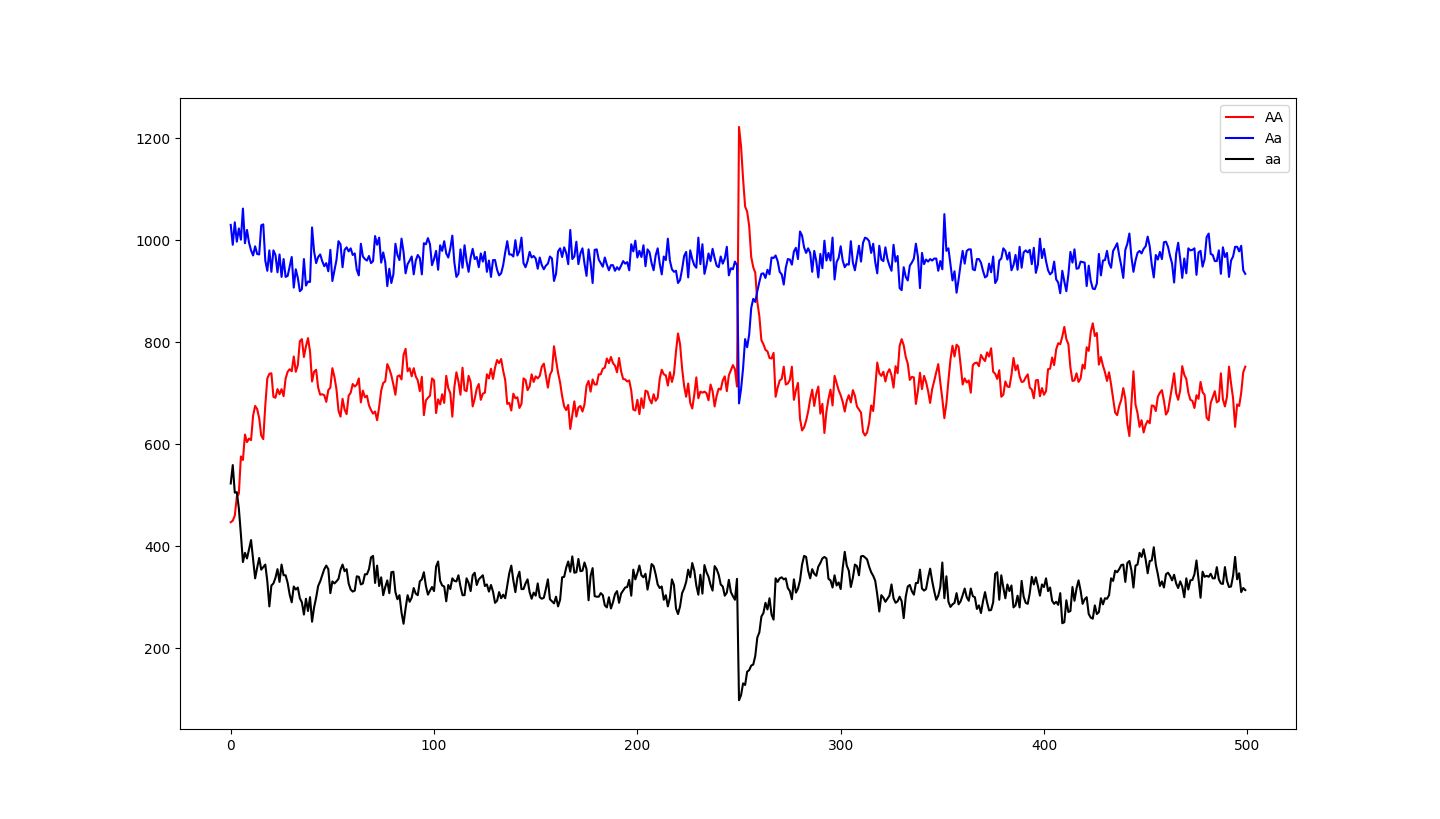
\includegraphics[width=0.7\linewidth]{sim5.png} 
\end{figure}	
\end{center}	
	
\end{frame}

\begin{frame}[t]{Why is equilibrium restored?}
	Equilibrium is restored because the AA are more likely to die than the Aa, so
	when the frequency of AA is very high the rate at which AA die is much higher
	than the rate at which AA are created by mating. As the frequency of AA goes
	down the rate at which AA die and are produced by mating equal each other.
	
\end{frame}

\begin{frame}[t]{An Equilibrium Constant}
	If I were to describe my situation in terms of reactions it would look like:
	$$\dom + \rec \rightleftharpoons \het$$
	The analogy is somewhat flawed, but what I mean is that there is some probability of an aa and a AA combining to make an Aa, and some probability of an Aa and an Aa combining to make either a AA or a aa.
	Then the "equilibrium constant" would be 
	$$\frac{[\het]}{[\dom][\rec]}.$$
	"Concentrations" should naturally be interpretted as frequencies.
	The fact that given the death probabilities of each genotype this is a constant means that it makes sense as an equilibrium constant. 

\end{frame}

\begin{frame}[t]{Some Intuition for the meaning of the Equilibrium constant}
	\begin{itemize}
		\item If this "equilibrium constant" is large then the forward reaction is favored. What this means here is that if Aa have a lower probability of dying then they will become prominent in the population.
		\item The analogy isn't perfect, because even if Aa are sure to survive while AA, aa are sure to die each year, then from the mating process about $\frac{1}{4}$ of the offspring from the all Aa population will be AA and $\frac{1}{4}$ will be aa.
		\item If this "equilibrium constant" is small, then either AA or aa will be very large. From my simulations this seems to mean that it is very likely that over time all other genotypes will die out eventually. This could be interpretted as the reaction going to completion.
	\end{itemize}
\end{frame}

\begin{frame}[t]{The End}
	
\begin{center}
	\begin{figure}
		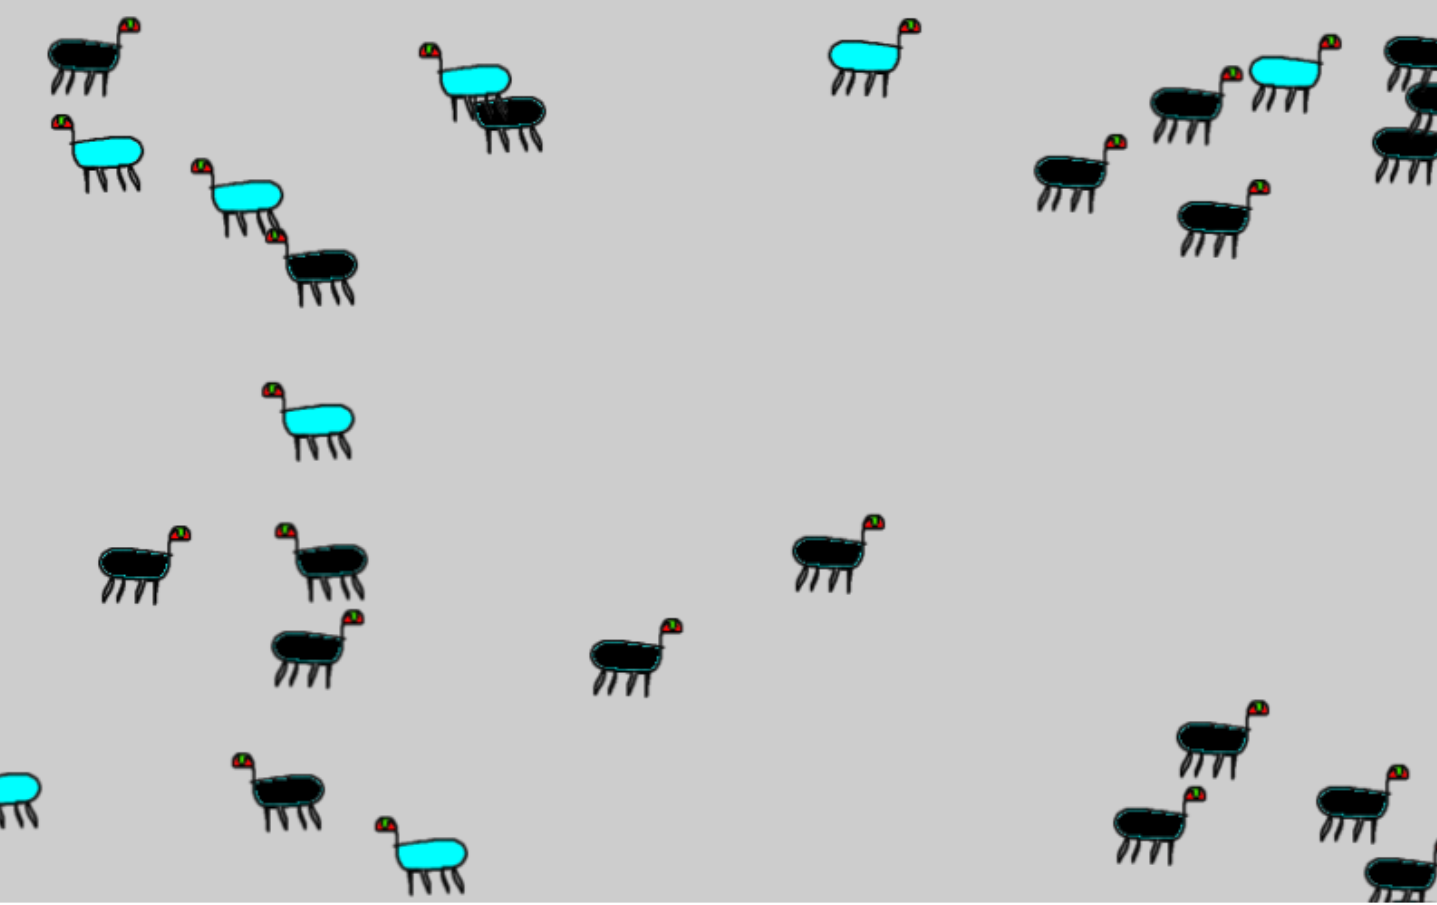
\includegraphics[width=0.9\linewidth]{gamePic.png} 
		\caption{The game version of the simulation}
\end{figure}	
\end{center}	

\end{frame}

\end{document}


